\section{Related Works}

Past research that address image and volume segmentation using sparse supervision can be roughly divided in two categories,
The first category, mainly focuses on computer vision techniques, while the second focuses on developping Machine Learning techniques.
In practice, both categories often overlap.

We now give an overview of the state-of-the-art in computer vision.
Next, we focus on \gls{ml} methods.


\subsection{Computer Vision Methods}
Another line of research focuses on the annotation protocol itself so as to complement the above efforts.
While the most tedious protocol requires that images be manually segmented at a pixel-level, many computer-vision approaches exist to facilitate this task.

Early contributions relied on the Active Contour model \cite{kass88}, which assumes that an initial contour is given and parameterized as the nodes of a spline curve, in this context called an elastic snake.
The segmentation problem is formulated as finding the deformation of the initial snake that minimizes an energy term.
In its simplest form, the energy term is composed of a term that determines the fitting of the snake to the edges of the image, while another term controls the smoothness of the snake.
The energy is then minimized using gradient descent.
Following works alleviate the problem of robustness brought by noisy edge maps by minimizing the Mumford-Shah functional \cite{chan01}, and parameterize the contour using the level-set method \cite{osher88}.

More recently, annotations in the form of scribbles were considered, where the annotator is asked to draw crude delineations of one or several objects of interest, along with a scribble on the background.
A first method that handles such kind of annotations relies on the Random-Walk algorithm \cite{grady06}.
The segmentation problem reduces to assigning to each unlabeled pixel a random-walker. The label of the latter pixel is then determined by the finding the label for which the walker has a maximum probability of reaching first.

Relying on the same annotation requirement, the graph-cut approach \cite{Boykov2006}
minimizes an Markov Random Field energy objective that considers unary terms (a scalar on each pixel), and a pairwise term that models the similarity of neighboring pixels.
Concretely, the image or volume is represented as a region adjacency graph where each pixel is assigned a node, and edges connect adjacent pixels.
Each annotated positive pixels is connected to a source node, while annotated negatives are connected to a sink node.
The energy minimization is then performed using the min-cut/max-flow algorithm \cite{goldberg88}.
Using the same algorithm, grab-cut \cite{rother04}, further simplifies the scribble-based annotation protocol by considering bounding-boxes around the object of interest, which provide crude labels on both foreground and background in a single stroke.
An illustration of the graph-cut framework is shown on Fig. \ref{fig:graphcut}.

\begin{figure}[!h]
  \centering
  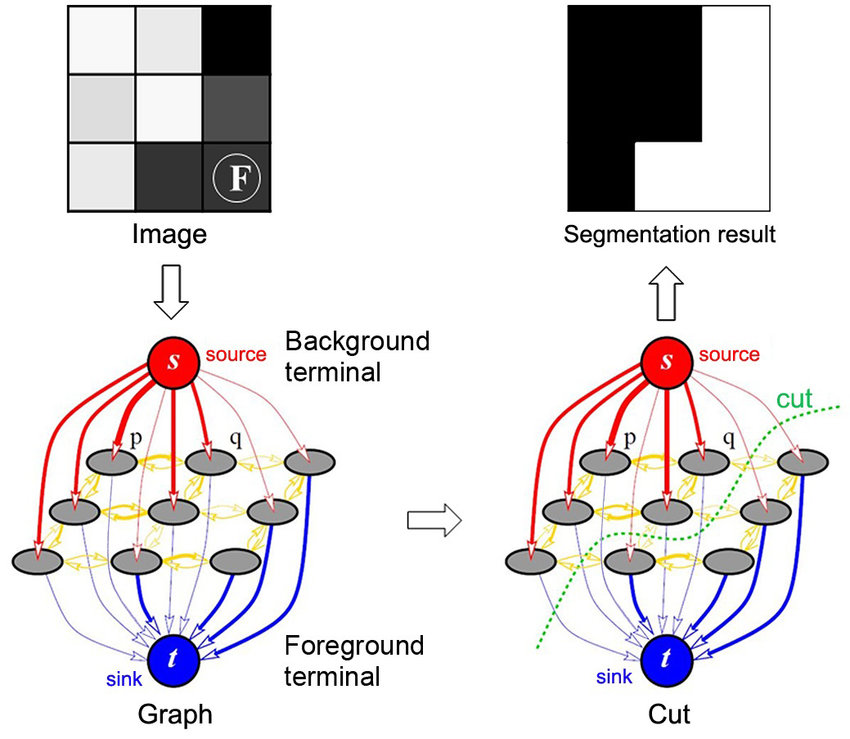
\includegraphics[width=8cm]{graphcut.jpeg}
  \caption{Min-cut/max-flow graph used for graph-cut segmentation. Taken from \cite{xiao17}.}
  \label{fig:graphcut}
\end{figure}

More recently, \cite{krahenbuhl11} proposed an inference strategy to apply a fully-connected \gls{crf} model to coarse pixelwise class-predictions, as a mean to enforce spatial coherence.
Similar to graph-cut, the latter minimizes an energy function that include unary and pairwise potentials, but considers that every pixel is connected all other pixels.
Fig. \ref{fig:crf} shows examples on natural images.

\subsection{Active Learning and Crowd-sourcing}
The problem of scarcity of labeled data can also be posed in the following manner:
Given a limited annotation budget, i.e. when only a few hours of annotation work can be provided, how can one make the best use of it?

\gls{al} \cite{settles09} considers semi-supervised learning scenarios, where abundant unlabeled data are available.
\gls{al} algorithms aim at selecting the unlabeled samples that are the most informative to the \gls{ml} model.
Conversely, \gls{al} assumes that many unlabeled samples represent redundant information to the late-stage \gls{ml} model.
In \cite{KonSznFua15}, authors devise a strategy to select unlabeled supervoxels of a 3D volume so as to segment volumes of various modalities.
The approach iteratively trains a classifier and takes its entropy as measure of uncertainty.
Combining the latter with a geometric prior, which takes into account intuitive rules on spatial coherence, they sample a batch of most uncertain samples.
The classifier is then re-trained using the newly annotated samples.

Crowd-sourcing, refers to the outsourcing of the annotation task to a high number of annotators \cite{orting19}.
Its use in the frame of medical imaging poses several limitations.
First, the difficulty of the annotation task can prohibit the effective use of crowd-sourcing, e.g when the structure of interest is hard to distinguish \cite{orting19}.
Another limitation is the nature of the data, i.e. one usually prefers to pre-classify brain scans and submit to workers the slices where tumors are present.
Last, one must usually integrate a test-task to ensure the competence of workers, or filter-out annotations provided by ``poorly performing'' workers \cite{park18}.

\subsection{Weakly supervised learning}
An important line of research, weakly supervised learning, endeavors to transpose sparse annotation protocol to the \gls{ml} field.
In \cite{dai15}, authors leverage bounding-box annotations to supervise the training of a \gls{cnn}.
As a follow-up work, \cite{lin16} uses scribbles as annotations.
In \cite{papandreou15}, authors train a \gls{cnn} for semantic segmentation of images by combining pixelwise semantic supervision with image-level supervision in the form of ``tags'' (dog, cat, ...).
Closely related to the present thesis is the work of \cite{bearman16}, who train a \gls{cnn} with a combination of image-level and point-wise supervision.
Concretely, annotations consists in a single 2D location on the object of interest, along with a semantic label corresponding to the class of the object.

A transversal line of research endeavored to combine the traditional graph-cut/\gls{crf} paradigm to \gls{dl} in an attempt to enforce spatial coherence into semantic segmentation models as a refinement step, a requirement that is not immediately achievable through standard loss functions.
The problem is generally formulated as follows: A \gls{dl} predicts the unary potentials, while a late-stage module generates the pairwise potentials and solves the energy objective.
In \cite{rajchl16}, authors leverage the fully-connected \gls{crf} inference procedure of \cite{krahenbuhl11} to segment lung and brain images from bounding-box annotations using a \gls{cnn}.
The \gls{cnn} of \cite{rajchl16} predicts the unary and pairwise potentials and minimize the energy function using a parameterized \gls{crf} using a \gls{rnn}, thereby allowing the parameters of the feature extractor and pairwise similarity model to be optimized in end-to-end fashion.
In \cite{wang18}, authors propose a framework that relie on two steps, where the first generates an initial delineation using a \gls{cnn}, which an annotator can modify manually by drawing scribbles.
Another \gls{cnn} generates refines the initial delineation by leveraging the geodesic distance transform \cite{criminisi08}, which combines the initial delineation and the users input.
Their pipeline is shown on Fig. \ref{fig:deepigeos}.

\begin{figure}[!h]
  \centering
  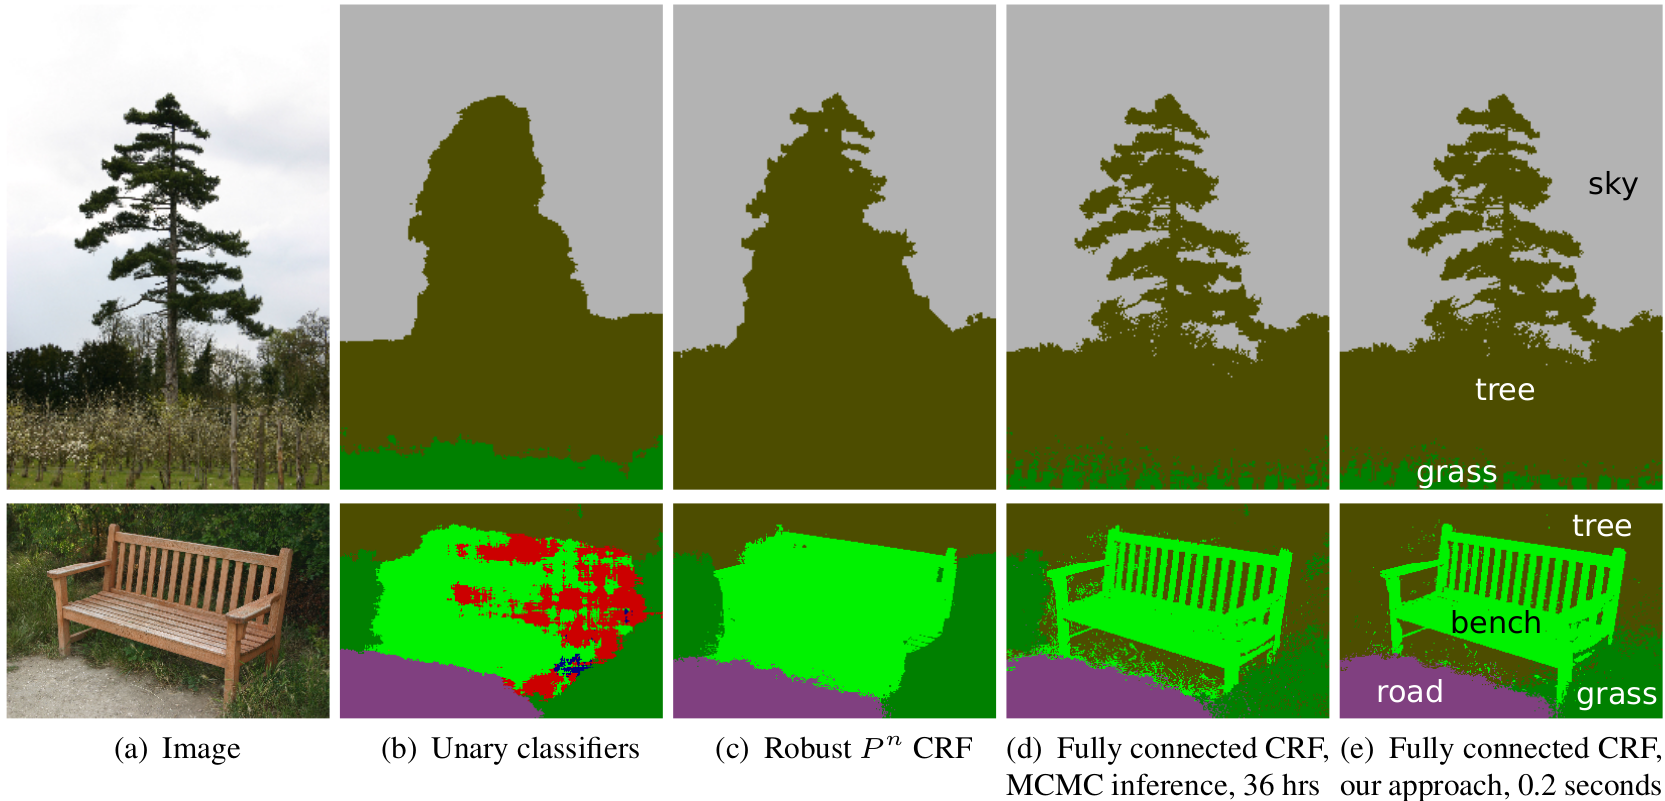
\includegraphics[width=12cm]{crf.png}
  \caption{Example segmentation using CRF on two images. (a) Input image (b) Response of the pixel-wise classifier (unary term) (c) Classification produced by the robust $P^{n}$ CRF \cite{kohli09} (d) Fully-connected CRF using Markov Chain Monte Carlo Inference (e) Approach of \cite{krahenbuhl11}. Taken from \cite{krahenbuhl11}.}
  \label{fig:crf}
\end{figure}

\begin{figure}[!h]
  \centering
  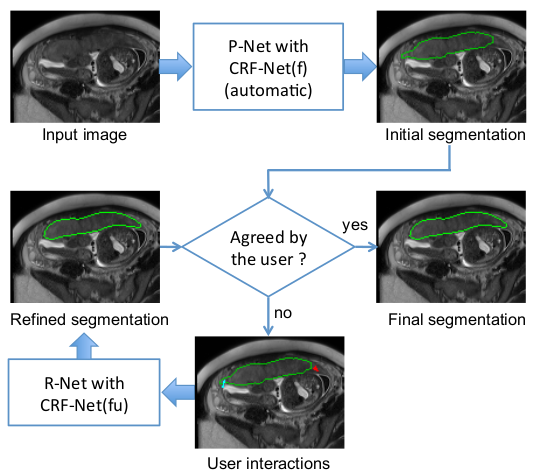
\includegraphics[width=8cm]{deepigeos.png}
  \caption{Deep Interactive Geodesic framework of \cite{wang18}. P-Net proposes an initial automatic segmentation that is refined by R-Net with user interactions indicating mis-segmentations. CRF-Net(f) is a
    back-propagatable CRF that uses freeform pairwise potentials.
    It is extended to be CRF-Net(fu) that employs user interactions as hard constraints. Taken from \cite{wang18}}
  \label{fig:deepigeos}
\end{figure}

Another trend in weakly supervised segmentation is the attention map paradigm.
The latter starts from a standard image-level classification \gls{cnn}, and considers that the response of late layers (before the classification layer), called \gls{cam}, can provide valuable cues on where the network is focusing.
In particular, Grad-CAM \cite{selvaraju17} proposes to generate segmentation maps by combining the activations of late layers with a weighting factor, computed using the backpropagated gradient.
In \cite{li18}, show that such attention maps, as provided by a \gls{cnn} trained only for classification, can be refined using a limited number of pixelwise annotated images.

More recently, adversarial techniques have been employed to semi-supervised semantic segmentation, as a mean to circumvent he computational burden at test time brought by the latter \gls{crf} approach.
In particular, the \gls{gan} approach \cite{goodfellow14} considers a \gls{cnn} that divides in two sub-networks: A generator, and a discriminator.
The first receives a random noise signal which it uses to generate an image that is as ``realistic'' as possible, while the second must distinguish images coming from the generator and real images.
In \cite{luc16}, authors argue that a spatial coherence refinement step similar in spirit to \gls{crf}, can be achieved through the \gls{gan} framework.
In particular, authors combine a standard segmentation network with a discriminator network,
where the latter must distinguish between the predicted label maps of the segmentation network and the groundtruth maps.
Both networks are then trained in parallel using a loss function that combines both objectives.


\subsection{Transfer Learning, Semi-supervised Learning, and Domain Adaptation}
\gls{tl} consists in using a \gls{ml} model trained for the task of interest, but using a training set of different nature than the targeted domain, e.g. train a \gls{cnn} to segment natural objects (trees, cars, ...) for the segmentation of surgical tools.
As pointed out by \cite{oliver18}, an important and implicit assumption in that context is that both datasets share similar data distributions.

\gls{ssl} is a broad category of \gls{ml} algorithm that combines traditional supervised learning tasks, where a scarce fully labeled training dataset is available, along with an abundant unlabeled dataset.
The latter can, under specific conditions, boost the performance of an \gls{ml} model trained with labeled dataset only, i.e. in a fully-supervised manner.
The basic idea is that the ML model may acquire knowledge of the data distribution from the unlabeled set.
Here again, one assumes that both data domains share similar distributions.
In \cite{ghafoorian17}, authors show experimentally that a \gls{nn} trained to segment tumors on MRI brain scans acquired in a given MRI protocol, perform poorly when transfered to another protocol, as the shape, intensities, and contrast level are inconsistent.

\gls{da} addresses the problem of adapting the model so as to take into account domain shift, i.e. the discrepancies between the training and target domain.
In \cite{perone19}, authors devise a strategy to segment MRI scans of spinal cords using a model trained with images taken at a specific field-of-view, and transfer to another field-of-view in an unsupervised fashion.
Their approach leverages data-augmentation to enforce a consistency between the augmented and pristine images of the unlabeled set, while jointly training with the labeled set with traditional cross-entropy loss.
On the same image modality, \cite{li20} resort to adversarial training. They jointly train a segmentation model and a discriminator wit shared weights. The discriminator is trained to discriminate between the source and target domain.

%%% Local Variables:
%%% mode: latex
%%% TeX-master: "../../main"
%%% End:
